\documentclass[12pt]{jsarticle}
%\documentclass[fleqn,twocolumn,10pt]{jsarticle}
	% [数式左揃え,ページ分割,フォントサイズ]{日本語用}
%\setlength{\mathindent}{1zw}
%\setlength{\columnsep}{3zw} 

\usepackage{listings}            % ソースコード用
\usepackage[dvipdfmx]{graphicx}  % 図の挿入用
\usepackage{amsmath,amssymb}     % 数式
\usepackage{mathrsfs}            % mathscr font
\usepackage{float}               % 図・表位置[H]
\usepackage{subcaption}          % subfigure/subtable可
\usepackage[dvipdfmx]{graphicx}  	% 図の挿入用\\
\usepackage[dvipdfmx]{color}
\usepackage[dvipdfmx]{hyperref}  % Link/URL
\usepackage{pxjahyper}           % "hyperref"の日本語文字化け対策
\usepackage{color,soul}          % highlight (sty file)
\usepackage{makeidx}             % 索引
\makeindex                       % 索引



% センターライン
\setlength{\columnseprule}{0.4pt}

% 行列matrixのサイズをスケーリングする
\newcommand\scalemath[2]{\scalebox{#1}{\mbox{\ensuremath{\displaystyle #2}}}}

% 日本語ハイライト
\newcommand{\HL}[1]{\hl{\mbox{#1}}}
%   ref: http://otoya8bit.hatenablog.jp/entry/2013/11/28/153226

% url custom
\hypersetup{
		colorlinks,  % これをtrueにすると何故かbuildしたとき画像(image)がpdfに表示されなくなったことがあった
    linkcolor=blue,
    filecolor=magenta,      
    urlcolor=cyan,
    bookmarksopen,
    bookmarksdepth=2,
    bookmarkstype=toc,  % toc link
%    linktocpage=true,   % tocのページ番号にリンクが現れる
    bookmarks=true,     % pdfにbookmarkを付与
    bookmarksnumbered=true,
    pdftitle={2018年 春 多変量解析},
    pdfauthor={pollenJP},
    pdfkeywords={多変量解析,multivariate,analysis},
    % 
    % ref
    % https://texwiki.texjp.org/?hyperref#h026c44c
    % book: [改訂第7番]LaTeX2 \epsilon 美文書作成入門
}


% table of contents config
\makeatletter
    \renewcommand*\l@subsection{\@dottedtocline{2}{3.8em}{4em}}
\makeatother
\title{2018年度 秋学期 ディジタル信号処理}
\author{A1678975 杉崎弘明 github @pollenjp}


% main
\begin{document}

    \maketitle

    \begin{abstract}
      レポート課題の図は,MatLabではなくPythonのnumpy,matplotlib等を用いて描画した.
      なお,このテキスト内で書いたコードは以下のgithubページから .ipynb の形でコードと出力結果を見ることができる.
      \url{https://github.com/pollenjp/Sophia_University_DSP_Discrete_Signal_Processing_report_201901}
	    \tableofcontents
	    \addtocontents{toc}{\hfill\textbf{Page}\par}
    \end{abstract}
    
    %--------------------------------------------------------------------------------
    % 
    %--------------------------------------------------------------------------------
    \section{課題} \label{課題}
      \subsection{課題内容} \label{課題内容}
      次のインパルス応答を有する LTI システムを考える
      \begin{align*}
        h [n] = \delta [n] + 2 \delta [n-1] + \delta [n-2]
      \end{align*}

      このシステムに対し,周波数が $f$ の正弦波を入力したときに出力振幅が何倍されるかを調べ,
      周波数を様々に変化させてこのフィルタの周波数特性( $20 \log10 |H|$ による対数振幅スペクトル) を求めよ.
      それを以下の理論特性と比較せよ.

      \begin{itemize}
        \item 20*log10(abs(fft(h,fs)))
        \item freqz(h,1)
      \end{itemize}

      ★オプション : 
      自分が選んだ音楽ファイルを上記のシステムにてフィルタ処理せよ. 処理前後の音楽を聴き比べ,どのような違いが感じられるか論ぜよ.

      
%--------------------------------------------------------------------------------
%--------------------------------------------------------------------------------
    \section{解答} \label{解答}
      \subsection{理想的なフィルタの周波数特性} \label{理想的なフィルタの周波数特性}
        $h[n]$ は因果的にするために右シフトされたものと考えられるが, シフトする前の $h[n]$ は以下の用になるので,それにフーリエ変換を行う.
        シフトしない変換は \ref{考察} で触れる.
        \begin{align*}
          h [n] &= \delta [n+1] + 2 \delta [n] + \delta [n-1] \\
          \text{連続化} h(x) &= \sum_{k=- \infty}^{\infty} h(k) \delta(x-k)\\
          H(e^{j \omega})
            &= \mathscr{F} \left[ h(x) \right] \\
            &= \mathscr{F} \left[ \sum_{k=- \infty}^{\infty} h(k) \delta(x-k) \right] \\
            &= \int_{x=-\infty}^{\infty} \sum_{k=- \infty}^{\infty} h(k) \delta(x-k) e^{-j \omega x} \mathrm{d} x \\
            &= \sum_{k=- \infty}^{\infty} h(k) \int_{x=-\infty}^{\infty} \delta(x-k) e^{-j \omega x} \mathrm{d} x \\
            &= \sum_{k=- \infty}^{\infty} h(k) e^{-j \omega k} \\
            &= \sum_{k=- \infty}^{\infty} \left( \delta [k+1] + 2 \delta [k] + \delta [k-1] \right) e^{-j \omega k} \\
            &= 1 \cdot e^{-j \omega \cdot (-1)} + 2 \cdot e^{-j \omega \cdot 0} + 1 \cdot e^{-j \omega \cdot 1} \\
            &= 1 \cdot e^{j \omega} + 2 + 1 \cdot e^{-j \omega} \\
            &= 1 \cdot ( \cos (\omega) + j \sin (\omega) ) + 2 + 1 \cdot ( \cos (\omega) - j \sin (\omega) ) \\
            &= 2 (1 + \cos (\omega)) \\
        \end{align*}
        
        これらの計算式により算出された $H(e^{j \omega}) = 2 (1 + \cos (\omega))$ をプロットするコードを以下に示す.
        プロットは図\ref{img-frequency_property_of_an_ideal_filter}に示す.
        
%--------------------------------------------------------------------------------
%--------------------------------------------------------------------------------
        \begin{lstlisting}[basicstyle=\ttfamily\footnotesize, frame=single]
import numpy as np
import matplotlib
import matplotlib.pyplot as plt
%matplotlib inline

seed=0
np.random.seed(seed)

# \omega と H(e^{j\omega}) のグラフ
fs = 16000              # サンプリング周波数:16kHz
_omega = np.arange(fs)
H_ejw = 2 * (1 + np.cos(2 * np.pi * (_omega / fs)))
###########################################################
matplotlib.rcParams['text.usetex']=True
fig = plt.figure(figsize=(15,5))
nrow, ncol = 1, 1
plot_idx = 0
############################################################
############################################################
plot_idx += 1
_x = _omega
_y = H_ejw
ax = fig.add_subplot(nrow, ncol, plot_idx)
ax.plot(_x, _y, color="black")
#ax.stem(freqs, amplitude_list,
#        linefmt="C0-" , markerfmt='o', basefmt='C3-')
_x = _omega
_y = np.ones_like(_omega)
ax.plot(_x, _y, color="black", linestyle="--")
ax.set_title(label="$H(e^{j\omega})$ frequency property",fontsize=15)
ax.set_xlabel(xlabel="freq : [Hz]",fontsize=15)
ax.set_ylabel(ylabel="$H(e^{j \omega})$",fontsize=15)
############################################################
############################################################
plt.subplots_adjust(wspace=0.2, hspace=0.4)
plt.show()
############################################################
matplotlib.rcParams['text.usetex']=False
				\end{lstlisting}
				
    		\begin{figure}[H]
    			\begin{center}
    				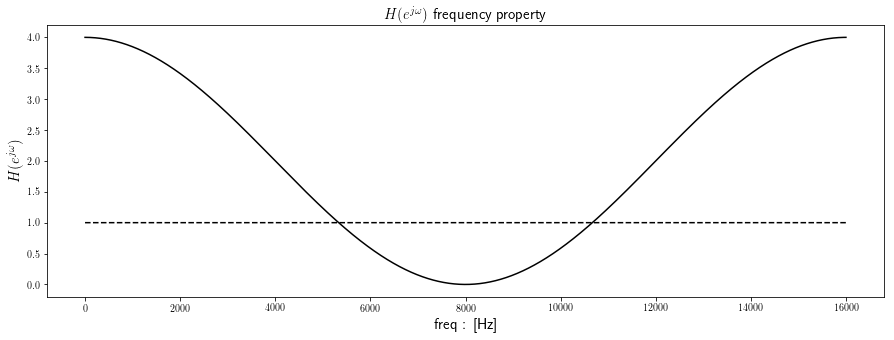
\includegraphics[width=1.0\columnwidth]{img/frequency_property_of_an_ideal_filter.png}
    				%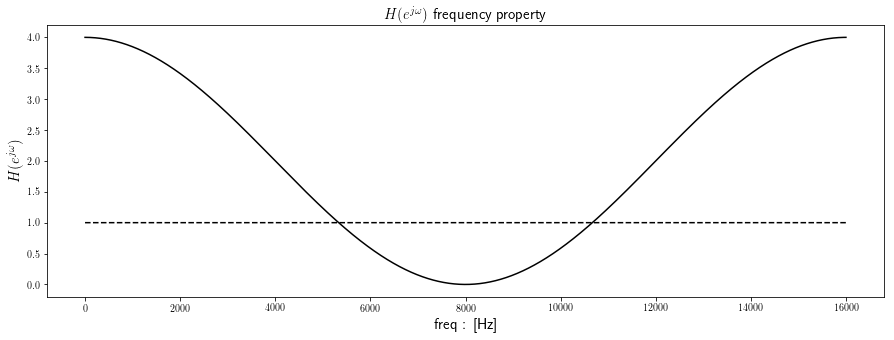
\includegraphics[width=10cm]{img/frequency_property_of_an_ideal_filter.png}
    				\caption{理想的フィルタの周波数特性}
    				\label{img-frequency_property_of_an_ideal_filter}
    			\end{center}
    		\end{figure}
    		
    		図\ref{img-frequency_property_of_an_ideal_filter} より,ローパスフィルタの特性を示すことがわかる.

%--------------------------------------------------------------------------------
%--------------------------------------------------------------------------------
        この周波数特性のグラフをパワースペクトルの常用対数表示で示す.
        \begin{align*}
          10 \cdot \log_{10} | H(e^{j \omega}) |^2 = 20 \cdot \log_{10} | H(e^{j \omega}) |
        \end{align*}
        以下にプロットのためのPython3コードを示し, 図\ref{img-ideal_20log10(abs(fft(h,fs)))}に図を示す.
        \begin{lstlisting}[basicstyle=\ttfamily\footnotesize, frame=single]
###########################################################
matplotlib.rcParams['text.usetex']=True
fig = plt.figure(figsize=(15,5))
nrow, ncol = 1, 1
plot_idx = 0
############################################################
############################################################
plot_idx += 1
_x = _omega[1000:7000]
_y = 20 * np.log10(H_ejw[1000:7000])
ax = fig.add_subplot(nrow, ncol, plot_idx)
ax.plot(_x, _y, color="black")
_x = _omega[1000:7000]
_y = np.zeros_like(_x)
ax.plot(_x, _y, color="black", linestyle="--")
ax.set_title(label="$20 * \log_{10}(|y|_{max}/|x|_{max})$",
             fontsize=15)
ax.set_xlabel(xlabel="freq : [Hz]",fontsize=15)
ax.set_ylabel(ylabel="$20 * \log_{10}(|y|_{max}/|x|_{max})$ [dB]",
              fontsize=15)
############################################################
############################################################
plt.subplots_adjust(wspace=0.2, hspace=0.4)
plt.show()
############################################################
matplotlib.rcParams['text.usetex']=False
				\end{lstlisting}

    		\begin{figure}[H]
    			\begin{center}
    				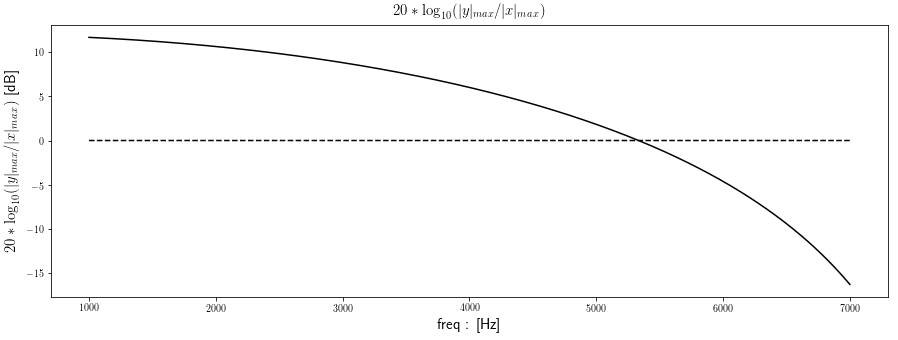
\includegraphics[width=1.0\columnwidth]{img/ideal_20log10(abs(fft(h,fs))).png}
    				\caption{理想的フィルタの周波数特性を対数グラフ表示}
    				\label{img-ideal_20log10(abs(fft(h,fs)))}
    			\end{center}
    		\end{figure}

%--------------------------------------------------------------------------------
%--------------------------------------------------------------------------------
      \subsection{各周波数に対して周波数特性を確認} \label{各周波数に対して周波数特性を確認}
        まずは周波数を1000Hzから7000Hzまでを100Hz刻みで取得し,各周波数に対して畳み込み処理を施す.
        \begin{lstlisting}[basicstyle=\ttfamily\footnotesize, frame=single]
fs = 16000              # サンプリング周波数:16kHz
t = np.arange(fs) / fs  # 離散時間 (1秒間)

freqs = list(np.arange(1000, 7001, 100))  # frequencyn
x_list = [ np.sin(2*np.pi*freq*t) for freq in freqs ]
				\end{lstlisting}

        \begin{lstlisting}[basicstyle=\ttfamily\footnotesize, frame=single]
# 畳み込み処理
h = np.array([1, 2, 1])

y_list = []

for freq, x in zip(freqs, x_list):
    y = np.convolve(a=x, v=h, mode="full")
    #y_list.append(y)
    # 後ほど左端は描画した時にグラフを歪めるので取り除く(比較する)
    # h のサイズが2なので両端ひとつずつだが,
    # サンプリング周波数と合わせるために先頭のみtrtimmingする
    y_trim_left = y[1:]
    y_list.append(y_trim_left)
				\end{lstlisting}
				
				ここで各周波数に対して振幅比を以下の指標で表す.
				
				\begin{align*}
				  20 * \log_{10}\left(\frac{|y|_{max}}{|x|_{max}}\right) \text{[dB]}
				\end{align*}
				
				コードとプロット(図\ref{img-frequency_property_from_each_freq})を以下に示す.
				( $y=1.0$ に直線を引いたのは後の考察で比較する際にわかりやすくするためである.)
				
        \begin{lstlisting}[basicstyle=\ttfamily\footnotesize, frame=single]
# 振幅倍率
amplitude_list = []
for freq, x, y in zip(freqs, x_list, y_list):
    dB = 20 * np.log10( np.abs(y).max() / np.abs(x).max() )
    amplitude_list.append(dB)
matplotlib.rcParams['text.usetex']=True
fig = plt.figure(figsize=(15,5))
nrow, ncol = 1, 1
plot_idx = 0
############################################################
############################################################
plot_idx += 1
ax = fig.add_subplot(nrow, ncol, plot_idx)
ax.plot(freqs, amplitude_list, color="black")
ax.stem(freqs, amplitude_list,
        linefmt="C0-" , markerfmt='o', basefmt='C3-')
ax.set_title(label="$20 * \log_{10}(|y|_{max}/|x|_{max})$",
             fontsize=15)
ax.set_xlabel(xlabel="freq : [Hz]",fontsize=15)
ax.set_ylabel(ylabel="$20 * \log_{10}(|y|_{max}/|x|_{max})$ [dB]",
              fontsize=15)
############################################################
############################################################
plt.subplots_adjust(wspace=0.2, hspace=0.4)
plt.show()
############################################################
matplotlib.rcParams['text.usetex']=False
				\end{lstlisting}

    		\begin{figure}[H]
    			\begin{center}
    				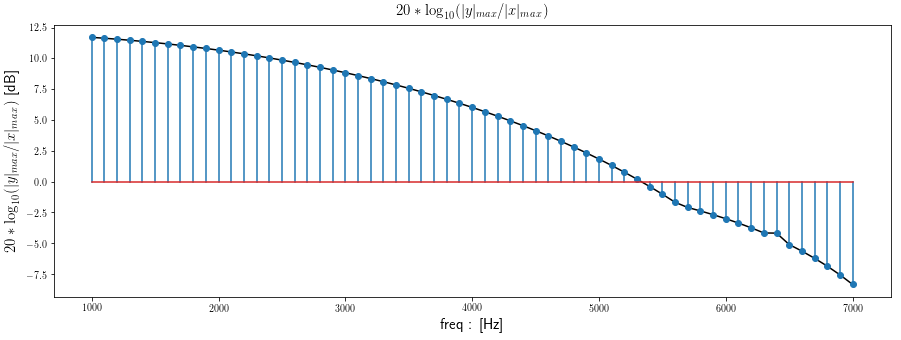
\includegraphics[width=1.0\columnwidth]{img/frequency_property_from_each_freq.png}
    				\caption{各周波数から求めた周波数特性}
    				\label{img-frequency_property_from_each_freq}
    			\end{center}
    		\end{figure}

%--------------------------------------------------------------------------------
%--------------------------------------------------------------------------------
      \subsection{考察} \label{考察}
        ローパスフィルタの形をしていることがわかり,
        理想フィルタにおいて $H(e^{j \omega}) = 1$ の周波数(5500Hz)あたりでは
        図\ref{img-frequency_property_from_each_freq} が $0.0$ になっていることがわかる.
        つまり,畳み込みが周波数領域における積であることが確認できる.
        
        また, \ref{理想的なフィルタの周波数特性} では $h[n]$ のシフトをずらして扱ったが,ずらさずに計算すると以下の用になる.
        $z$ 変換によっても求まるので合わせて以下に載せておく.
        
        \begin{align*}
          h [n] &= \delta [n] + 2 \delta [n-1] + \delta [n-2] \\
          \text{連続化} h(x) & \sum_{k=- \infty}^{\infty} h(k) \delta(x-k)\\
          H(e^{j \omega})
            &= \mathscr{F} \left[ h(x) \right] \\
            &= \mathscr{F} \left[ \sum_{k=- \infty}^{\infty} h(k) \delta(x-k) \right] \\
            &= \int_{x=-\infty}^{\infty} \sum_{k=- \infty}^{\infty} h(k) \delta(x-k) e^{-j \omega x} \mathrm{d} x \\
            &= \sum_{k=- \infty}^{\infty} h(k) \int_{x=-\infty}^{\infty} \delta(x-k) e^{-j \omega x} \mathrm{d} x \\
            &= \sum_{k=- \infty}^{\infty} h(k) e^{-j \omega k} \\
            &= \sum_{k=- \infty}^{\infty} \left( \delta [k] + 2 \delta [k-1] + \delta [k-2] \right) e^{-j \omega k} \\
            &= 1 \cdot e^{-j \omega \cdot 0} + 2 \cdot e^{-j \omega \cdot 1} + 1 \cdot e^{-j \omega \cdot 2} \\
            &= 1 + 2 \cdot e^{-j \omega} + e^{-2j \omega} \\
            &= (1 + e^{-j \omega}) + e^{-j \omega} \cdot (1 + e^{-j \omega}) \\
            &= (1 + e^{-j \omega})^2 \\
          \text{z変換} H(z)
            &= \sum_{n=0}^{\infty} h[n] z^{-n} \\
            &= \sum_{n=0}^{\infty} \delta[n] z^{-n}
              + \sum_{n=0}^{\infty} 2 \delta[n-1] z^{-n}
              + \sum_{n=0}^{\infty} \delta[n-2] z^{-n} \\
            &= 1 + 2z^{-1} + z^{-2} \\
          H(e^{j \omega})
            &= 1 + 2 e^{-j \omega} + e^{-2j \omega}) \\
            & \ \ \ \ \ \  (\because z=e^{-j \omega} \text{を代入}) \\
            &= (1 + e^{j \omega})^2 \\
          | H(e^{j \omega}) |
            &= | 1 + 2 \cdot (\cos(\omega) - j \sin(\omega))  + (\cos(2\omega) - j\sin(2\omega)) | \\
            &= | (1 + 2 \cos(\omega) + \cos(2\omega)) - j ( 2\sin(\omega) + \sin(2\omega)) | \\
            &= ( (1 + 2 \cos(\omega) + \cos(2\omega)) - j ( 2\sin(\omega) + \sin(2\omega)) )^{\frac{1}{2}} \\
        \end{align*}
        
        すると, $h'[n] = \delta[n] + \delta[n-1]$ を $z$ 変換すると $H'(z) = 1 + z^{-1}$ になるので
        フーリエ変換 ($z=e^{j\omega}$) したものは $H(e^{j\omega}) = 1 + e^{-j\omega}$ となる.
        これより,$h[n] = h'[n] + h'[n-1]$ の関係があり,
        今回の $H(e^{j\omega}) = (1 + e^{-j\omega})^2$ と比較すると $2$ 乗になっていることがわかる.
        
        オプションとして,授業中に渡されたmusic.wavファイルに $h[n]$ を畳み込んでみた.
        音楽を聴き比べると畳み込みをしたあとの音はラジオのようなノイズがかなり多く入りとてもききづらかったが,
        処理前の音楽には聞こえていたシンバルの音が処理後には聞こえていないように感じた.
        これは畳み込みにより高い周波数のシンバルの音が除外されたためである.
        また,全体的に音がかなり大きめに感じられたが,
        それは畳み込み処理により低周波数の信号(5500Hzよりも小さい信号)が増幅されたためと考えられる.
        
        Python3のコードを最後に示す.
        
        \begin{lstlisting}[basicstyle=\ttfamily\footnotesize, frame=single]
fs, x = scipy.io.wavfile.read(filename="./music.wav")
h = np.array([1, 2, 1])
y = np.convolve(a=x, v=h, mode="full")
# サンプリング周波数と合わせるために先頭のみtrtimmingする
y_trim_left = y[1:]
# yの音声ファイル作成
_wave_file = "./music_convolved_report.wav"
_y = np.float32(y)
wavfile.write(filename=_wave_file,
              rate=fs,  # サンプリング周波数
              data=_y)
				\end{lstlisting}
				

\end{document}

